\chapter{Message Construction}
An AYDP message is constructed from three basic components; a header, a data section, and a checksum. The checksum at the end of each sentence is a single byte which is the XOR of all of the bytes in the sentence (excluding itself). This checksum byte is only intended to allow the recipient to ensure that the message is complete, not to re-build any missing data.

\begin{figure}[H]
  \centering
  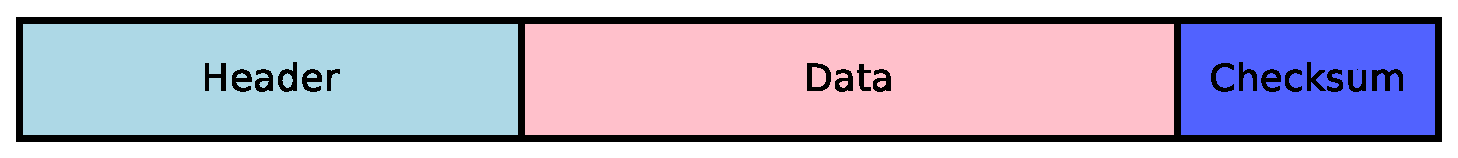
\includegraphics[width=1.0\textwidth]{Figures/protocolBasicLayout.eps}
  \label{figure:msg:basicProto}
  \caption{Basic protocol layout}
\end{figure}

The header is 27 bytes long and contains the message type and length as shown in table \ref{table:msg:header}.

\begin{table}[H]
  \centering
  \begin{tabular}{ c c c c }
  Byte &          Content    & Data Type & Length  \\
       &                     &           & (bytes) \\
\hline
   1   &  Start (0xFF)       &   uint8   &    1    \\
   2   &  Message Type       &   uint8   &    1    \\
   3   &  Message Length     &   uint32  &    4    \\
   7   &  Seconds from epoch &   int64   &    8    \\
   19  &  Milliseconds into current second & int64 & 8 \\
  \end{tabular}
  \caption{Header Contents}
  \label{table:msg:header}
\end{table}

For message types $\geq 127$ (i.e. where the MSB of the message type is high) the timing data is omitted. This is termed an expedited message, and the header becomes only six bytes long. This is used to transfer high-speed data where the transmission time is secondary to the data rate. Any message can be expidited, simply by adding 127 to the message identifier.

\section{Transmission limitations}

The expidited message form is useful for serial links, but it should be noted that ethernet and WiFi links will hit packet rate limits before the bandwidth limits, except in the case of extremely large messages, where expedited transfer will make little difference anyway.
